\documentclass{article}
\title{COMS W4115
	Assignment 1}
\author{Programming Languages and Translators\medskip\\
	Xijiao Li (xl2950)}
\usepackage{listings}
\usepackage{amsmath}
\usepackage[utf8]{inputenc}
\usepackage{listings}
\usepackage{color}
\usepackage{setspace}
\usepackage{enumitem}
\usepackage{graphicx}
\usepackage{dirtytalk}
\usepackage{tikz}
\usetikzlibrary{automata, positioning, arrows}

\renewcommand{\baselinestretch}{1.1} 


\definecolor{dkgreen}{rgb}{0,0.6,0}
\definecolor{gray}{rgb}{0.5,0.5,0.5}
\definecolor{mauve}{rgb}{0.58,0,0.82}
\def\code#1{\texttt{#1}}


\lstset{
	%language=Python,
	aboveskip=3mm,
	belowskip=3mm,
	showstringspaces=false,
	columns=flexible,
	basicstyle={\small\ttfamily},
	numbers=none,
	numberstyle=\tiny\color{gray},
	commentstyle=\color{dkgreen},
	stringstyle=\color{mauve},
	breaklines=true,
	breakatwhitespace=true,
	tabsize=3,
	mathescape
}

\begin{document}
	\tikzset{
		->, % makes the edges directed
		>=stealth, % makes the arrow heads bold
		node distance=2.5cm, % specifies the minimum distance between two nodes. Change if necessary.
		every state/.style={thick, fill=gray!10}, % sets the properties for each ’state’ node
		initial text=$ $, % sets the text that appears on the start arrow
	}
	\pagenumbering{gobble}
	\maketitle
	
	\newpage
	\pagenumbering{arabic}
	\subsection*{Problem 1}
	\subsubsection*{a.}
	1*0(01*0+1)*\\
	$\epsilon$ is not valid since it has 0 number of \say{0}'s.
	\subsubsection*{b.}
	0*1*1\\
	$\epsilon$ is not valid since it is not ending with a \say{1}.
	
	\subsection*{Problem 2}
	From the graph we know that the NFA recognizes all strings that contain two 0’s, between which there can optionally be a substring $s$ and $s$ must has length equal to a multiple of 3. A regular expression for the NFA is (0+1)*0((0+1)(0+1)(0+1))*0(0+1).
	
	
	\subsection*{Problem 3}
	\subsubsection*{a.}
	$coms4115: \ [a-z][a-z 0-9]^*$\\
	Based on maximal munch, we will pick $[a-z][a-z 0-9]^*$, since it can fully cover the input.
	
	\subsubsection*{b.}
	$while: [a-z][a-z 0-9]^*$\\
	Based on maximal munch, we pick $[a-z][a-z 0-9]^*,\ for|while|if |else$, since they can fully cover input. Based on the rule of thumb, we pick $[a-z][a-z 0-9]^*$ due to its higher priority.
	
	\subsubsection*{c.}
	$123abc: \  [0-9]^*[a-z],\ [a-z][a-z 0-9]^*$\\
	We need to do partition here, since no rule can cover the full input. Based on maximal munch, we pick $[0-9]^*[a-z]$ first since it can cover the most number of characters \say{123a} among other rules. Then we have \say{bc} left, and based on maximal munch, we pick $[a-z][a-z 0-9]^*$.
	
	\subsubsection*{d.}
	$dictionary: [a-z][a-z 0-9]^*$\\
	Based on maximal munch, we pick $[a-z][a-z 0-9]^*,\ dictionary$, since they can fully cover input. Based on the rule of thumb, we pick $[a-z][a-z 0-9]^*$ due to its higher priority.
	
	\subsubsection*{e.}
	The empty string: none\\
	No rules apply, since all rules require the valid inputs to contain at least one character.
	
	\subsection*{Problem 4}
	\subsubsection*{a.}
	$ (p+q)^*+(p+r)^*+(q+r)^*$
	
	\subsubsection*{b.}
	NFA $M = (Q,\ \Sigma,\ \delta,\ q_0,\ F)$ is defined as:
	\begin{align*}
	&Q = \{ q1, q2, q3, q4, q5 \}\\
		&\Sigma = \{ p, q, r \}\\
		&S = q_1\\
		&F = \{ q_2, q_3, q_4 \}\\
		&\delta:
	\end{align*}
	           \begin{center}
	           	\begin{tabular}{|c |c| c| c|} 
	           		\hline
	           		state \textbackslash input & $p$ & $q$ & $r$ \\ [0.5ex] 
	           		\hline
	           		$q_1$ & $q_2, q_3$ & $q_2, q_4$ & $q_3, q_4$ \\ 
	           		\hline
	           		$q_2$ & $q_2$ & $q_2$ & $q_5$ \\
	           		\hline
	           		$q_3$ & $q_3$ & $q_5$ & $q_3$ \\
	           		\hline
	           		$q_4$ & $q_5$ & $q_4$ & $q_4$ \\
	           		\hline
	           		$q_5$ & $q_5$ & $q_5$ & $q_5$ \\
	           		\hline
	           	\end{tabular}
	           \end{center}
    The state machine is as follows:
	\begin{center}
		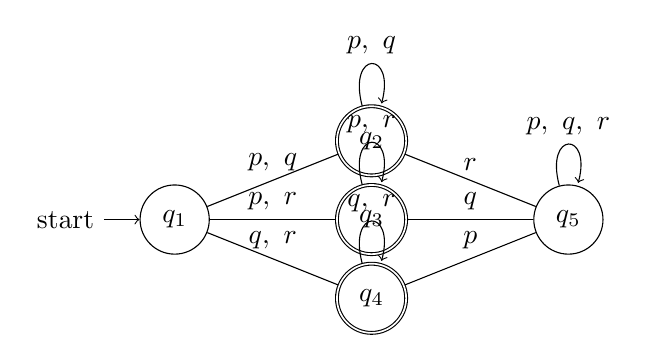
\begin{tikzpicture}
			\node[state, initial] (q1) {$q_1$};
			\node[state, accepting, right of=q1,  xshift=1.5cm] (q3) {$q_3$};
			\node[state, accepting, above of=q3] (q2) {$q_2$};
			\node[state, accepting, below of=q3] (q4) {$q_4$};
			\node[state, right of=q3,  xshift=1.5cm] (q5) {$q_5$};
			\draw    
						(q1) edge[above] node{$p,\ q$} (q2)
						(q1) edge[above] node{$p,\ r$} (q3)
						(q1) edge[above] node{$q,\ r$} (q4)
						(q2) edge[loop above] node{$p,\ q$} (q2)
						(q3) edge[loop above] node{$p,\ r$} (q3)
						(q4) edge[loop above] node{$q,\ r$} (q4)
						(q5) edge[loop above] node{$p, \ q,\ r$} (q5)
						(q2) edge[above] node{$r $} (q5)
						(q3) edge[above] node{$q$} (q5)
						(q4) edge[above] node{$p$} (q5);
		\end{tikzpicture}
	\end{center}

	\subsubsection*{c.}
	The transition table is as follows:
	 \begin{center}
		\begin{tabular}{|c |c| c| c|} 
			\hline
			state \textbackslash input & $p$ & $q$ & $r$ \\ [0.5ex] 
			\hline
			$q_1$ & $q_2, q_3$ & $q_2, q_4$ & $q_3, q_4$ \\ 
			\hline
			$q_2, q_3$ & $q_2, q_3$ & $q_2, q_5$ & $q_3, q_5$ \\ 
			\hline
			$q_2, q_4$ & $q_2, q_5$ & $q_2, q_4$ & $q_4, q_5$ \\ 
			\hline
			$q_3, q_4$ & $q_3, q_5$ & $q_4, q_5$ & $q_3, q_4$ \\ 
			\hline
			$q_2, q_5$ & $q_2, q_5$ & $q_2, q_5$ & $q_5$ \\ 
			\hline
			$q_3, q_3$ & $q_3, q_5$ & $q_5$ & $q_4, q_5$ \\ 
			\hline
			$q_4, q_5$ & $q_5$ & $q_4, q_5$ & $q_4, q_5$ \\ 
			\hline
			$q_5$ & $q_5$ & $q_5$ & $q_5$ \\
			\hline
		\end{tabular}
	\end{center}
The state machine for DFA is as follows:
	\begin{center}
		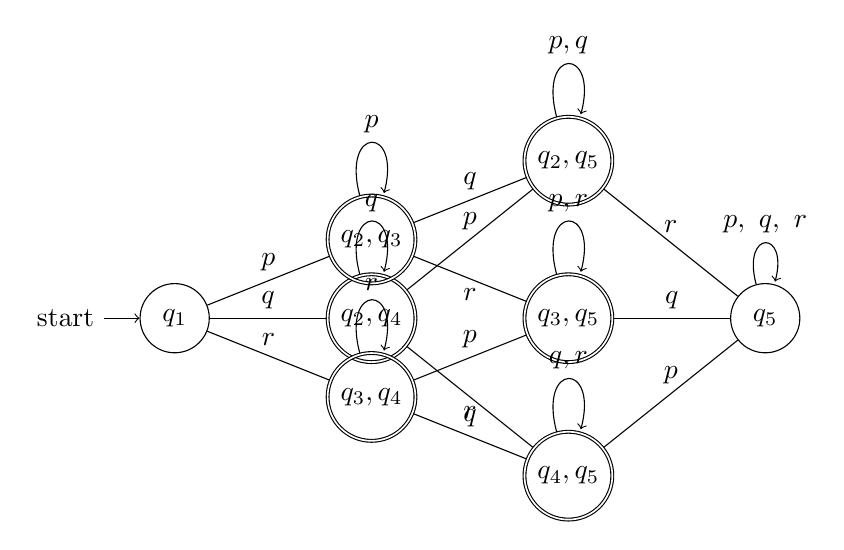
\begin{tikzpicture}
			\node[state, initial] (q1) {$q_1$};
			\node[state, accepting, right of=q1,  xshift=1.5cm] (q3) {$q_2, q_4$};
			\node[state, accepting, above of=q3] (q2) {$q_2, q_3$};
			\node[state, accepting, below of=q3] (q4) {$q_3, q_4$};
			\node[state, accepting, right of=q3,  xshift=1.5cm] (q6) {$q_3, q_5$};
			\node[state, accepting, above of=q6, yshift=1cm] (q5) {$q_2, q_5$};
			\node[state, accepting, below of=q6, yshift=-1cm] (q7) {$q_4, q_5$};
			\node[state, right of=q6,  xshift=1.5cm] (q8) {$q_5$};
			\draw    
			(q1) edge[above] node{$p$} (q2)
			(q1) edge[above] node{$q$} (q3)
			(q1) edge[above] node{$r$} (q4)
			(q2) edge[loop above] node{$p$} (q2)
			(q3) edge[loop above] node{$q$} (q3)
			(q4) edge[loop above] node{$r$} (q4)
			(q2) edge[above] node{$q$} (q5)
			(q2) edge[below] node{$r$} (q6)
			(q3) edge[above] node{$p$} (q5)
			(q3) edge[below] node{$r$} (q7)
			(q4) edge[above] node{$p$} (q6)
			(q4) edge[above] node{$q$} (q7)
			(q5) edge[loop above] node{$p,q$} (q5)
			(q6) edge[loop above] node{$p,r$} (q6)
			(q7) edge[loop above] node{$q,r$} (q7)
			
			(q8) edge[loop above] node{$p, \ q,\ r$} (q8)
			(q5) edge[above] node{$r $} (q8)
			(q6) edge[above] node{$q$} (q8)
			(q7) edge[above] node{$p$} (q8);
		\end{tikzpicture}
	\end{center}
	
	\subsubsection*{5.}
	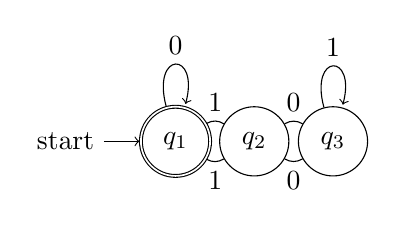
\begin{tikzpicture}
		\node[state, initial, accepting] (q1) {$q_1$};
		\node[state, right of=q1] (q2) {$q_2$};
		\node[state, right of=q2] (q3) {$q_3$};
		
		\draw (q1) edge[loop above] node{0} (q1)
		(q1) edge[bend left, above] node{1} (q2)
		(q3) edge[loop above] node{1} (q3)
		(q2) edge[bend left, above] node{0} (q3)
		(q2) edge[bend left, below] node{1} (q1)
		(q3) edge[bend left, below] node{0} (q2);
	\end{tikzpicture}\\
	Let $x$ denote the scanned binary input.\\
	$q_1$ refers to the state that $x \mod 3 \equiv 0$, $q_2$ refers to the state that  $x \mod 3 \equiv 1$, and $q_3$ refers to the state that  $x \mod 3 \equiv 2$. So $q_1$ will be our initial state as well as the accepting state, and we begin to calculate the reminder from 0.\\
	Suppose that the current $x$ has a reminder of 0.
	\begin{enumerate}
		\item the next input is 0: $x$ is doubled.\\ $2x \mod 3 \equiv 0$, and it will stay at $q_1$.
		\item the next input is 1: $x$ is doubled and incremented by 1.\\ $2x+1 \mod 3 \equiv 1$, and it will go to $q_2$.
	\end{enumerate}
Suppose that the current $x$ has a reminder of 1.
\begin{enumerate}
	\item the next input is 0: $x$ is doubled.\\
	$2x \mod 3 \equiv = 2$, and it will go to $q_3$.
	\item the next input is 1: $x$ is doubled and incremented by 1.\\
	$2x + 1 \mod 3  \equiv 0$, and it will go to $q_1$.
\end{enumerate}
Suppose that the current $x$ has a reminder of 2.
\begin{enumerate}
	\item the next input is 0: $x$ is doubled.\\
	$2x \mod 3 \equiv 1$, and it will go to $q_2$.
	\item the next input is 1: $x$ is doubled and incremented by 1.\\
	$2x + 1 \mod 3 \equiv 2$, and it will stay at $q_3$.
\end{enumerate}
\end{document}